%\newcommand{\eps}{\epsilon}
\newcommand{\Pmax}{p_\text{max}} 	
\newcommand{\Hint}{H_{int}}
\newcommand{\kbar}{\bar{k}}
\newcommand{\Delk}{\Delta}
\newcommand{\Sumk}{\Sigma}
\newcommand{\Qrot}{Q_{pq}(\tau_s)}
\newcommand{\shapecor}{\mathcal{S}}
\newcommand{\ampcor}{\mathcal{A}}
\newcommand{\totalcor}{\mathcal{E}}
\newcommand{\threeLs}{L_p(\kbar_1)L_q(\kbar_2)L_r(\kbar_3)}
\newcommand{\threePs}{P_p(\kbar_1)P_q(\kbar_2)P_r(\kbar_3)}
\newcommand{\threeQs}{Q_p(k_1)Q_q(k_2)Q_r(k_3)}
\newcommand{\Lbasic}{\mathcal{P}_0}
\newcommand{\Linvk}{\mathcal{P}_1}
\newcommand{\Lnsinv}{\mathcal{P}^{n_s}_1}
\newcommand{\Lnsboth}{\mathcal{P}^{n_s}_{01}}
\newcommand{\Linvksq}{\mathcal{P}_2}
\newcommand{\Lns}{\mathcal{P}^{n_s}_2}
\newcommand{\Fbasic}{\mathcal{F}_0}
\newcommand{\Finvk}{\mathcal{F}_1}
\newcommand{\Finvksq}{\mathcal{F}_2}
\newcommand{\quadpot}{V_{\phi^2}(\phi)}
%\newcommand{\threeqs}{q_p(\kbar_1)\,q_r(\kbar_2)\,q_s(\kbar_3)}
\newcommand{\threeqs}{q_p(k_1)\,q_r(k_2)\,q_s(k_3)}
\newcommand{\threeqstilde}{q_{\tilde{p}}(k_1)\,q_{\tilde{r}}(k_2)\,q_{\tilde{s}}(k_3)}
\newcommand{\kmin}{{k_\text{min}}}
\newcommand{\kmax}{{k_\text{max}}}
\newcommand{\fnl}{f_{NL}}
\newcommand{\fnllocal}{f^{local}_{NL}}
\newcommand{\fnlequil}{f^{equil}_{NL}}
\newcommand{\fnlortho}{f^{ortho}_{NL}}

\chapter{Introduction II: Probing Inflation}\label{chapter:intro_bispectra}
In this chapter we will review details of the bispectrum, including how it is predicted
by an inflationary scenario and connected to the $\cmb$ sky.
We will point out where our methods diverge from previous work,
briefly discuss the computational complexity of the $\cmb$ calculation, and
the approximations that have previously been used to make this tractable.


The primordial bispectrum is one of the main
characteristics used to distinguish between models of inflation. While it is well
known that the physics of inflation must have been extremely close
to linear, and the initial seeds of structure it laid down
drawn from a probability distribution that was
very close to Gaussian, there is expected to have been some level of coupling
between the Fourier modes of the perturbations.
In the simplest example of an inflation model this is
expected to be unobservable~\cite{Maldacena},
but the possibility remains that inflation was driven by
more complex physics that may have left an observable imprint on our universe today.
Some models of inflation have interactions that predict non-Gaussian
correlations at observable levels. This can happen through
self-interactions~\cite{px_burrage,dbi_in_the_sky},
interactions between multiple fields~\cite{Byrnes_2010, Gao_turn,
achucarro_multifield1, achucarro_multifield2, achucarro_robust_16, achucarro_natural,
achucarro_quad_viability, achucarro_gsr_cs_14, achucarro_cs_reduction_13,
achucarro_gong_cs_corr, achucarro_cs_12, achucarro_eft, curvaton_comprehensive},
sharp features~\cite{adshead, gsr, step_novaes}
and periodic features~\cite{flauger_pajer_resonant, Pajer_2013, Meerburg_2012, Meerburg_osc, Meerburg_2010,
Barnaby_2011, Peiris_2013, Easther_2013, Cabass_2018, Behbahani_2011}.
Another observable consequence of primordial non-Gaussianity
that has been studied,
through which it could possibly be probed, is the generation of primordial black
holes~\cite{pbh_byrnes, pbh_young, pbh_franciolini, pbh_passaglia}.
%Ultra slow-roll is a regime that has been explored~\cite{usr_chowdhury,usr_pattison,
%usr_dimopoulos,usr_martin}


We will focus on non-Gaussianity from a single field in this thesis,
however inflation scenarios with more than one field are an
active field of research.
In these models, which are motivated by string theory considerations~\cite{achucarro_multifield1},
non-linearities of interactions between fields during inflation
can generate observably large non-Gaussian signals.
This is in part because they can evade the squeezed limit consistency condition~\cite{sqz_consistency}.
The extra degrees of freedom in these scenarios can also generate bispectrum shapes not usually
seen in single-field models (for example, see recent work in~\cite{RP_2, Fumagalli_2019}).
Multi-field models are a prime target for future work---the
methods outlined in this thesis have been implemented
and tested for single-field models,
though they are expected to generalise to this case.


If the fundamental physical model of inflation is a single field,
then the non-linearities of the self-interactions of that field may have
produced observably large non-Gaussian signatures~\cite{Tolley_2010, achucarro_eft}.
Detecting these signatures in the $\cmb$ bispectrum requires an understanding
of their form~\cite{Komatsu_2005}, which motivates the study of these dynamics.
Models of inflation that can produce observably large non-Gaussian signatures,
and are therefore constrained by the current experimental bounds~\cite{Planck_NG_2018},
include string theory-inspired models such as $\dbi$ inflation~\cite{dbi_silverstein}
and axion-monodromy~\cite{axion_monodr_review_09, Flauger_2014}
(which gives large non-Gaussianity through the resonance mechanism).


There is an extensive literature on the details of the calculation
of bispectra from models of inflation~\cite{chen_easther_lim_1,chen_easther_lim_2,chen_ng_0605,seery_ng_0503,px_burrage,adshead,flauger_pajer_resonant,features_bartolo,bdy_passaglia}.
Multi-field models can produce large
correlations between modes of very different scales;
non-canonical kinetic terms can reduce the sound speed of the perturbations,
boosting both the smooth non-Gaussian correlations, and any
features which may be present~\cite{dbi_adshead,dbi_in_the_sky,warp_features_dbi,dbi_silverstein,dbi_step_miranda,chen_folded_resonant,osc_avila};
effectively single-field models with imaginary sound speeds can generate a bispectrum
mostly orthogonal to the usual equilateral and local templates~\cite{RP_1}.


However, understanding the inflationary prediction is only the first part of the process.
The computational challenge of using these predictions to translate
$\cmb$ data into constraints on specific inflation scenarios has been tackled by
various methods.
Much progress has been made by coarse-graining
the model space, using a small number of approximate representative templates,
and leveraging the simplifying characteristic of separability
with respect to the three parameters of the bispectrum~\cite{Komatsu_2005, Munchmeyer_2014}.


The primordial bispectrum is the Fourier equivalent of the
three-point correlator of the primordial curvature perturbation.
If this field is Gaussian, the bispectrum vanishes, so
it is a valuable measure of the interactions in play during inflation.
If some inflation model predicts a bispectrum that is sufficiently well approximated by
the standard separable templates, the constraints on those standard templates
can be translated into constraints on the parameters of the model.
The fact that the amplitudes of all primordial templates estimated thus far from the CMB
are consistent with zero has already provided such constraints
in certain scenarios~\cite{Planck_NG_2015, Planck_NG_2018}.
With the high-precision \planck~data, and data from forthcoming experiments
such as the Simons Observatory (SO)~\cite{simons}
and CMB-S4~\cite{abazajian2016cmbs4}, robust pipelines must be developed to
extract the maximum amount of information possible,
by bypassing the approximations and
limitations of previous methods.


Constraining an arbitrary template using previous methods has been difficult
due to the nature of bispectrum estimation in the CMB and
LSS~\cite{lss_baldauf,lss_karagiannis,chen_future_lss,Scoccimarro_2012}.
Our aim in this work is to develop the inflationary part
of a pipeline to allow to efficiently test a much broader range of models.
In this work, we explore shapes arising from tree-level effects in single field models.
We do this numerically, allowing quantitative results for a broad
range of models, and avoiding extra approximations.
Our general aim is to apply the Modal philosophy of~\cite{FergShell_1,FergShell_2,FergShell_3}
to calculating primordial bispectra.
This Modal philosophy is a flexible method that has broadened the range of constrained
bispectrum templates, by expanding them in a carefully chosen basis.
The Modal estimator is thus capable of constraining
non-separable templates, while the $\ksw$ estimator~\cite{Komatsu_2005}, for example, cannot.


To do this, we will exploit the intrinsic separability of the
tree-level in-in formalism to apply the Modal methods at the level of inflation.
Expressing the primordial bispectrum in a separable
basis expansion turns out to lead to an increase in the efficiency
of the calculation at the primordial level.
However, the main advantage is still that
expressing the primordial shape function
in this way reduces the process of bispectrum estimation in the CMB to a
cost which (while large) need only be paid once per basis,
not per scenario.
The details of the bispectrum estimation part of
the pipeline will be detailed in~\cite{Sohn_2021}.


A proof of concept of this approach at the primordial level was presented in~\cite{Funakoshi}.
We go beyond the work of~\cite{Funakoshi} both in developing the choice of basis
(the feasibility of the method depending vitally on the chosen basis
achieving sufficiently fast convergence in a broad range of interesting models)
and in the methods we use to allow us to go to much higher order in our primordial expansion,
allowing us to apply the method to feature bispectra for the first time.


\section{Perturbations about the background}
    %We can get a lot of information on the evolution of the perturbations
    %from observations, and that tells us about the history of universe,
    %which tells us about its content, etc\ldots
    We begin by discussing the details of the perturbations.
    The action for the perturbations is derived by
    %working in a general gauge
    %(using the ADM formalism) and
    splitting the relevant quantities into a background
    part and a small perturbation, which we can parameterise
    for the inflaton $\phi$ and the metric $g_{\mu\nu}$ as
    \begin{align}
        \phi(t,\vecx)=\bar{\phi}(t)+\delta\phi(t,\vecx), \qquad g_{\mu\nu}=\bar{g}_{\mu\nu}+\delta g_{\mu\nu}
    \end{align}
    where $\bar{g}_{\mu\nu}$ is the unperturbed metric defined in~\eqref{flrw_metric}.
    In the uniform density gauge we have (neglecting tensor modes)
    \begin{align}
        \delta \phi=0, \qquad h_{ij}=a^2 e^{2\zeta} \delta_{ij}
    \end{align}
    where $h_{ij}$ is the spatial part of the metric.
    %The relation between $\zeta$ in uniform density gauge and
    %$\delphi$ in spatially flat gauge is
    %\begin{align}
    %    \zeta=-\frac{\delphi}{\sqrt{2\varepsilon}a}.
    %\end{align}
    The second order action for the perturbations in this gauge can be found to be
    \begin{align}\label{zeta_action}
        S_{2} = \int d^3x dt~\frac{a\varepsilon}{c_s^2}\left(a^2\dot{\zeta}^2-c_s^2\left(\partial\zeta\right)^2\right)
    \end{align}
    Defining $v=-z\zeta$ and switching to conformal time we can rewrite~\eqref{zeta_action} as
    \begin{align}\label{v_action}
        S_{2} = \frac{1}{2}\int d^3x d\tau \left[{\left(\frac{d v}{d \tau}\right)}^2-c_s^2\left(\partial v\right)^2+\frac{1}{z}\frac{d^2z}{d\tau^2}v^2\right]
    \end{align}
    where
    \begin{align}\label{z_defn}
        z^2 = \frac{2a^2\varepsilon}{c_s^2} = a^2\frac{\rho+P}{\left(c_sH\right)^2}.
    \end{align}
    In terms of $v$, we can recognise the dynamics as that of a
    canonically normalised scalar field, oscillating
    with a frequency that changes as the universe expands.
    The sound speed $c_s$~\eqref{sound_speed_definition} is
    the propagation speed of the perturbations.
    This defines a sound horizon, $c_s/H$---as the modes cross this sound
    horizon they freeze.
    Expanding the mass, we find
    \begin{align}
        %\frac{z''}{z} = 2{\left(aH\right)}^2\left(1+\frac{\eta}{2}-\varepsilon_s\right)\left(1+\frac{\eta-2\epscs-2\varepsilon+2\eta'-4\epscs'}{4}\right)
        %\frac{1}{z}\frac{d^2z}{d\tau^2} = 2{\left(aH\right)}^2\left(1+\ldots\right)
        \frac{1}{z}\frac{d^2z}{d\tau^2} \approx 2{\left(aH\right)}^2
    \end{align}
    where we have neglected terms that are slow-roll suppressed.
    The evolution of the perturbations is therefore well approximated using
    $\frac{1}{z}\frac{d^2z}{d\tau^2} = 2{\left(aH\right)}^2$,
    unless the evolution deviates from the slow-roll behaviour.

    \subsection{Evolution of the perturbations}\label{pert_evol}
    %https://nms.kcl.ac.uk/eugene.lim/AdvCos/lecture2.pdf
    %https://www.mpi-hd.mpg.de/lin/events/group_seminar/inflation/schmidt.pdf
    Varying the second order action~\eqref{zeta_action}, we can calculate the equation of motion
    of the perturbations.
    In terms of derivatives with respect to $N$, we obtain
    \begin{align}\label{modefneqn_zeta_N}
        {\zeta_k}'' + (3-\varepsilon+\eta-2\epscs){\zeta_k}'+\left(\frac{kc_s}{aH}\right)^2\zeta_k=0.
    \end{align}
    We can see that at late times, when $kc_s\ll aH$, $\zeta_k$ will freeze.
    This conservation of $\zeta$ outside the horizon~\cite{Lyth_conserved} is an
    important property\footnote{
    Systems with multiple degrees of freedom have $\zeta$ evolving even outside
    the horizon. See~\cite{Christopherson_2009} for a discussion on how this relates
    to non-adiabatic pressure in inflation models with non-canonical kinetic terms.}.
    It is useful as it means that $\zeta_k$ will then be frozen during the transition from inflation to the
    usual radiation dominated period, and we need only pick up the evolution again once it
    re-enters the horizon in the well-understood radiation era.


    From~\eqref{v_action}, in conformal time, we obtain the Mukhanov-Sasaki equation
    \begin{align}\label{modefneqn_tau}
        \frac{\partial^2 v_k}{\partial \tau^2} + \left(c_s^2k^2 - \frac{1}{z}\frac{d^2 z}{d \tau^2}\right)v_k = 0
    \end{align}
    however, this is not ideal as $c_s$ depends on time.
    Instead, let us use $\tau_s$~\eqref{tausdef} as our time parameter.
    If we follow~\cite{Hu_2011} and define
    \begin{align}\label{y_defn}
        y_k=\sqrt{2kc_s}v_k,
    \end{align}
    we obtain
    \begin{align}\label{modefneqn_tau_s}
        \frac{\partial^2 y_k}{\partial \tau_s^2} + \left(k^2 - 2\left(\frac{aH}{c_s}\right)^2(1+\ldots)\right)y_k = 0
    \end{align}
    where ``\ldots'' represents terms which are slow-roll suppressed.
    %where again \ldots~represents terms which are slow-roll suppressed.


    At early times, well before crossing the sound horizon at $c_sk=aH$,
    we have $k\gg aH/c_s$. We can see that the equation of motion becomes
    \begin{align}
        \frac{\partial^2 y_k}{\partial \tau_s^2} + k^2 y_k \approx 0
    \end{align}
    and we can clearly see that the solutions look like $y_k\propto e^{\pm ik\tau_s}$.


    \subsection{Early time behaviour}
    %\subsubsection{Quantizing the perturbations}
    We now wish to quantize the perturbations. We expand $v$ as
    \begin{align}\label{operator_expansion}
        v(\tau,\vecx) &= \int\frac{d^3\veck}{(2\pi)^3}\left[
            v_k(\tau)\hat{a}_\veck e^{i\veck\cdot\vecx}+
            v^*_k(\tau)\hat{a}^{\dagger}_\veck e^{-i\veck\cdot\vecx}
        \right]\\
            &= \int\frac{d^3\veck}{(2\pi)^3}\left[
            v_k(\tau)\hat{a}_\veck +
            v^*_k(\tau)\hat{a}^{\dagger}_{-\veck}
        \right]e^{i\veck\cdot\vecx}
    \end{align}
    where $v_k(\tau)$ and $v^*_k(\tau)$ satisfy~\eqref{modefneqn_tau}.
    The creation and annihilation operators satisfy
    \begin{align}\label{creation_annihilation_commutator}
        \left[\ahat_{\veck},\ahat^{\dagger}_{\veck'}\right] = (2\pi)^3\delta^{(3)}(\veck-\veck').
    \end{align}
    Taking the commutator of $v$ and its conjugate momentum $\pi=\frac{dv}{d\tau}$
    we can obtain the canonical commutator
    \begin{align}
        \left[v(\tau,\vecx),\pi(\tau,\mathbf{y})\right] &=
        \int \frac{d^3 \veck}{(2\pi)^3}\left(v_k\pi^*_k-\pi_kv^*_k\right)e^{i\veck\cdot(\vecx-\mathbf{y})}\\
        &= i \delta^{(3)}(\vecx-\mathbf{y})
    \end{align}
    if we demand that $v_k\pi^*_k-\pi_kv^*_k=i$.
%\subsubsection{Initial conditions for the perturbations}
    %We can define the vacuum state by $\ahat_{\veck}\left| 0\right>=0$.
    %Demanding this to be an eigenstate of $H$ forces $\pi_k=\pm ikv_k$.
    %Choosing the lowest energy state\ldots
    %and this is known as the Bunch-Davies vacuum.
    We notice that if we quantize $y$
    (defined in~\eqref{y_defn}), its Fourier modes
    should behave like a free field in Minkowski space with respect to $\tau_s$
    when they are deep in the horizon.
    Demanding this early time behaviour of $y_k$
    gives us the Bunch-Davies vacuum
    \begin{align}\label{bd_ic}
        v_k = \frac{1}{\sqrt{2{c_s}k}}e^{-ik\tau_s}
    \end{align}
    when $\frac{{c_s}k}{aH}\rightarrow \infty$.


    \subsection{Late time behaviour}
    %We can write the solution to the equations
    %of motion in terms of the Hankel function $H^{(2)}_i$ as~\cite{px_burrage}
    %\begin{align}
    %    \zeta_k = \frac{1}{2a}\sqrt{\frac{\pi}{2}}\sqrt{\frac{-\tau_s}{zc_s}}H^{(2)}_{\nu}\left[-k\tau_s\right].
    %\end{align}
    %where $\nu = \frac{3}{2}+\varepsilon+\frac{\eta}{2}+\frac{\epscs}{2}$


    %At late times we can use the limit
    %\begin{align}
    %    \lim_{x\rightarrow 0}H^{(1)}_\nu(x)\rightarrow-\frac{i}{\pi}\Gamma(\nu)\left(\frac{x}{2}\right)^{-\nu}.
    %\end{align}
    %From this limiting behaviour we can calculate the power spectrum predicted by
    %a $P(X,\phi)$ model, as a function of time and $k$.
    %What we find is that the time dependence
    %of the prefactor $H^2/(4zc_s^3)$ is precisely canceled out by the time dependence
    %of the limiting behaviour of the Hankel function, as expected.
    %This means we can obtain the final power spectrum by evaluating
    %it separately for each $k$. In fact, we choose to evaluate the asymptotic expression
    %at sound-horizon crossing $c_sk=aH$. Note that we are \textit{not} evaluating
    %$\zeta_k\zeta^*_k$ at horizon crossing---we are evaluating the
    %late-time asymptotic expression for that quantity there.


    Taking the slow-roll parameters as constant, we can obtain a simple approximate solution
    to~\eqref{modefneqn_zeta_N}
    \begin{align}\label{uk_solution}
        \zeta_k(\tau) = \frac{H}{\sqrt{4\varepsilon c_s k^3}}\left(1-ik\tau_s\right)e^{i k\tau_s}.
    \end{align}
    Treating the solution more carefully, one finds
    \begin{align}
        P_\zeta(k) = \frac{H^2}{4\varepsilon c_s k^3}
    \end{align}
    where the right-hand side is evaluated at $c_sk=aH$,
    defining the scale dependence of the result.
    This is enhanced by a factor of $c_s$ compared to the
    usual canonical power spectrum.
    For a review and discussion of corrections see~\cite{px_burrage}.


%The dimensionless power spectrum $\primpowerspec$~\eqref{primpowerspec_defn}
The power spectrum is typically parameterised as
\begin{align}
    P_\zeta(k) = A_s \left(\frac{k}{k_*}\right)^{n_s-1}.
\end{align}
The scalar spectral index $n_s$ can then be found to be
\begin{align}
n_s-1 = -2\varepsilon-\eta-\varepsilon_s
\end{align}
at leading order in slow-roll.


    For completeness, we note some possible points of notational confusion.
    In~\cite{px_burrage} the definition $s^{there}=d\ln c_s/dN$ is used, however we refer to this
    quantity (as we defined in~\eqref{slowrollparams}) as $\epscs$.
    In~\cite{Hu_2011}, the quantity referred to as $s$ is the integral of the sound speed
    with respect to conformal time---we refer to this quantity as $\tau_s$,
    which we defined in~\eqref{tausdef}.
    In~\cite{warp_features_dbi}, $\tau_s^{here}$ is also referred to as $s$,
    but $\epscs^{here}$ is referred to as $\sigma_1$.
    This is summarised in Table~\ref{tab:notation}.


\begin{table}[h!]
  \begin{center}
    \begin{tabular}{ccccc}
        \toprule
        Here & Definition &~\cite{px_burrage}&~\cite{Hu_2011} &~\cite{warp_features_dbi}\\
        \midrule
        $\tau_s$ &~\eqref{tausdef} & ~ & $s$ & $s$ \\
        $\epscs$ &~\eqref{slowrollparams} & $s$ & ~ & $\sigma_1$ \\
        $z$ &~\eqref{z_defn} & $\varepsilon/c_s^2$ & ~ & ~ \\
        \bottomrule
    \end{tabular}
    \caption{
        Notation summary and comparison for some inflationary parameters
        used in the literature.
    }\label{tab:notation}
  \end{center}
\end{table}


    \section{The power spectrum}\label{sec:power_spec_estimator}
    The fractional temperature anisotropies of the $\cmb$ can be decomposed in spherical
    harmonics $Y_{lm}$ as follows
    \begin{align}
        \frac{\Delta T}{T}(\hat{\mathbf{n}}) &= \sum_{l,m} a_{lm}Y_{lm}(\hat{\mathbf{n}}).
    \end{align}
    If we demand the statistics are invariant under rotation, it can be shown that
    \begin{align}
        \left<a_{lm}a^*_{l'm'}\right> &= \delta_{ll'}\delta_{mm'}C_l.
    \end{align}
    We can project the three dimensional inhomogeneities onto the $\cmb$ sky,
    using the Rayleigh plane wave expansion and the addition theorem
    for spherical harmonics. Writing $\vecx=r\hat{\vecn}$,
    \begin{align}
        e^{i\veck\cdot\vecx} &= \sum_l i^l(2l+1)j_l(kr)P_l(\hat{\veck}\cdot\hat{\vecn})\\
                    &= 4\pi\sum_{l,m}i^l j_l(kr)Y^*_{lm}(\hat{\veck})Y_{lm}(\hat{\vecn})\label{addition_expan}
    \end{align}
    where $j_l(x)$ is the spherical Bessel function.
    Expanding the fractional temperature fluctuations
    $\frac{\Delta T}{T}(\vecx)$ in Fourier modes,
    and then expanding the factor $e^{i\veck\cdot\vecx}$ using~\eqref{addition_expan},
    we find
    \begin{align}
        a_{lm} &= 4\pi i^l\int\frac{d^3k}{(2\pi)^3}\frac{\Delta T}{T}(\veck)j_l(k\chi_*)Y^*_{lm}(\hat{\veck})
    \end{align}
    where $\chi_*$ the comoving distance to last scattering.
    Then on large scales, we find
    \begin{align}\label{sachs_cl_example}
        C_l &\approx 4\pi\int d\ln k~\frac{\primpowerspec(k)}{25}{\left[
            j_l(k\chi_*)
            \right]}^2.
    \end{align}
    The factor of $1/5$ comes from the relation between the fractional temperature
    fluctuations and the primordial curvature perturbations on large scales. These are the scales
    that are sufficiently large that we can neglect acoustic oscillations during the
    radiation dominated epoch, leaving inhomogeneous gravitational redshifting
    (the Sachs-Wolfe effect) as the dominant contribution.
    The spherical Bessel function encodes the fact that a three dimensional
    wave of a given wavelength intersects the sphere at multiple different angular separations.


    For large scales, where there was not enough time for oscillations
    before recombination,
    the term $\left(j_l(k\chi_*)/5\right)^2$ acts as a transfer
    function that simply encodes the projection effects.
    For smaller scales where the physics is more complicated this would be encoded in
    some more general transfer function $\Delta_l(k)$
    \begin{align}\label{eqn:transfer_function}
        C_l &= 4\pi\int d\ln k~\primpowerspec(k)
            \Delta_l(k).
    \end{align}


    We can write down an estimator for this angular power spectrum.
    Since $C_l$ depends only on $l$, we can
    use all the values of $m$ for each $l$
    \begin{align}
        %\left<TT\right> &= ?\\
        %\left<a_{lm}a_{l'm'}\right> &= ?\\
        \hat{C}_l &= \frac{1}{2l+1}\sum_{m=-l}^{l} a_{lm} a^*_{lm}.
    \end{align}
    The variance of this estimator is given by
    \begin{align}
        var\left(\hat{C}_l\right) = \frac{2}{2l+1} C^2_l,
    \end{align}
    which reflects the fact that multipoles with higher $l$ have
    more independently drawn modes that we can observe.


    For $\primpowerspec(k)=A_s$, i.e.\ a perfectly scale invariant power spectrum,
    we can use that
    \begin{align}
        \int_0^{\infty}d\ln x~j_l^2(x) = \frac{1}{2l(l+1)}
    \end{align}
    to evaluate the expression for the large scale power spectrum~\eqref{sachs_cl_example}.
    We find that $l(l+1)C_l\propto \text{const}$, i.e.\ that on large scales
    (small $l$) this quantity is independent of $l$.


    %For intermediate scales, the acoustic oscillations and the Doppler effect
    %becomes relevant, and the transfer function additionally encodes this processing
    %\begin{align}
    %    C_l \approx 4\pi\int d\ln k~\primpowerspec(k){\left[
    %        \frac{(\Theta_0+\psi)(\eta_*,\mathbf{k})}{\mathcal{R}(\mathbf{k})}j_l(k\chi_*)
    %        -\frac{v_\gamma(\eta_*,\mathbf{k})}{\mathcal{R}(\mathbf{k})}j'_l(k\chi_*)
    %        \right]}^2.
    %\end{align}


\section{The primordial bispectrum}
    \subsection{The shape function}
The primordial bispectrum is usually written as:
\begin{align}\label{bispectrum_definition}
{
\left< \zeta_{\bf{k_1}}\zeta_{\bf{k_2}}\zeta_{\bf{k_3}} \right>
= (2\pi)^3\delta^{(3)}(\mathbf{k_1}+\mathbf{k_2}+\mathbf{k_3})B(k_1,k_2,k_3)
}
\end{align}
The delta function comes from demanding statistical homogeneity;
demanding statistical isotropy restricts the remaining dependence to the magnitudes of the vectors.
We denote the magnitude of $\mathbf{k_i}$ as $k_i$.
This leaves us with a function of three parameters,
$k_1,k_2,k_3$.
It is useful to define the dimensionless shape function
\begin{align}\label{shapefn}
    S(k_1,k_2,k_3) = (k_1k_2k_3)^2B(k_1,k_2,k_3).
\end{align}
As we saw in Section~\ref{corr_functions}
the bispectrum is only defined where the triangle condition
\begin{align}\label{triangle_condition}
    \mathbf{k_1}+\mathbf{k_2}+\mathbf{k_3} &= 0,
\end{align}
is satisfied, which implies that the triangle inequality must hold
\begin{align}\label{triangle_inequality}
    k_1+k_2 &\geq k_3~\text{and cyclic perms}.
\end{align}
Thus, we will occasionally speak of the bispectrum as a function of types
of triangles---for example, when the three magnitudes are
equal they form an equilateral triangle, and when one is much smaller than
the other two, a squeezed triangle.
The space of configurations we are interested in is therefore
reduced from the full cube $[\kmin,\kmax]^3$
to a~\textit{tetrapyd} (illustrated in Figure~\ref{fig:tetrapyd_diagram}),
which is defined as the intersection of that cube with the
tetrahedron that satisfies~\eqref{triangle_inequality}.
This has important implications that we will explore in
Chapter~\ref{chapter:decomp}. 
\begin{figure}[h!]
\centering
    \subfloat{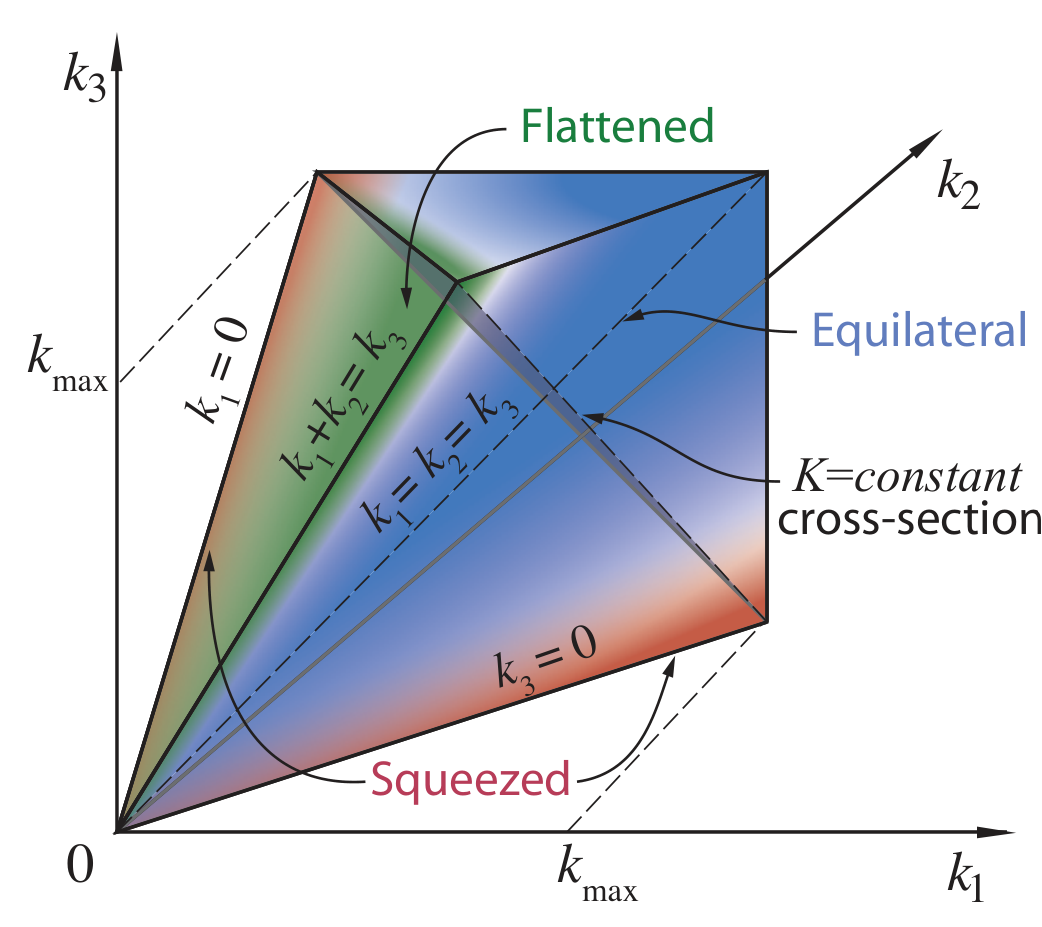
\includegraphics[width=\columnwidth]{plots/tetrapyd_3d_colour_split.png}}
\caption{
    Half of the tetrapydal region on which the bispectrum is defined,
    along with the various limits commonly discussed in the literature.
    We thank Paul Shellard for providing this figure.
}\label{fig:tetrapyd_diagram}
\end{figure}


The amplitude of a bispectrum shape is usually
quoted in terms of some amplitude parameter $\fnl^F$.
We can schematically define $\fnl^F$ for some template $F$ as follows:
\begin{equation}\label{def:fnl}
{
B^{F}(k_1,k_2,k_3) = \fnl^{F}\times F(k_1,k_2,k_3)
}
\end{equation}
where $F$ contains the dependence on the $k$-configuration.
This will be discussed further in later sections,
here we will merely note
%This definition coincides with the definitions of
%$\fnllocal$, $\fnlequil$ and $\fnlortho$
%when $F$ is (respectively) the local (see~\eqref{local_shape}),
%equilateral (see~\eqref{equil_shape}) and orthogonal templates,
%as defined in~\cite{Planck_NG_2013, Planck_NG_2015}.
that a distinction is sometimes made between the ``scale dependence''
of the bispectrum, meaning the dependence on $k_1+k_2+k_3$, and the ``shape dependence'',
meaning the dependence on each $k_i$ separately, for fixed $k_1+k_2+k_3$.


\section{Models}\label{sec:interactions}
We consider the same basic models as in~\cite{Funakoshi}.
Firstly, a quadratic potential
\begin{align}\label{eq:quadratic_potential}
    \quadpot = \frac{1}{2}m^2\phi^2
\end{align}
with a canonical kinetic term.
We will also consider a non-canonical model in detail, the $\dbi$ model.
    The $\dbi$ model has kinetic term
\begin{align}\label{eq:dbi_action}
    S_{\dbi}=\int d^4x\sqrt{-g}\left(-\frac{1}{f(\phi)}\left(\left(1+f(\phi)\partial_\mu\phi\partial^\mu\phi\right)^{\frac{1}{2}}-1\right)-V(\phi)\right),
\end{align}
and we choose
\begin{align}\label{eq:dbi_warp}
    f(\phi)=\frac{\lambda_{\dbi}}{\phi^4},\qquad
    V(\phi)=V_0-\frac{1}{2}m^2\phi^2,\qquad
    m=\sqrt{\beta_{IR}}H_{i}
\end{align}
where $\lambda_{\dbi}$, $\bir$ and $V_0$ are constants which
(along with the initial value of $\phi$, $\phi_0$) define the scenario in question.
$H_i$ is the Hubble parameter evaluated at the initial time.
This is in line with~\cite{Bean_ir_dbi, Chen_dbi}.


The energy-momentum tensor in~\eqref{einstein_equations}, in terms of the matter Lagrangian $\mathcal{L}_m$,
is given in~\eqref{gr_energy}.
%For a $P(X,\phi)$ model this evaluates to
%\begin{align}
%    T_{\mu\nu} &= g_{\mu\nu}P(X,\phi)+P_{,X}(X,\phi)\partial_{\mu}\phi\partial_{\nu}\phi\\
%            &\approx g_{\mu\nu}P(X,\phi)-2X\delta_{0\mu}\delta_{0\nu}P_{,X}(X,\phi).
%\end{align}
    Following~\cite{Christopherson_2009, mukhanov_1999},
    we can then use this to calculate the useful quantities
    \begin{align}
        P(X, \phi) &= -\frac{1}{f(\phi)}\left(\sqrt{1-2f(\phi)X}-1\right)-V(\phi)\\
        %P,_X(X, \phi) &= \frac{1}{\sqrt{1-2f(\phi)X}}\\
        %\rho(X, \phi) &= \frac{X}{\sqrt{1-f(\phi)X}}-P(X,\phi)\\
        %            &= \frac{1}{\sqrt{1-f(\phi)X}}(P+V)+V\\
        \rho(X, \phi) &= \frac{1}{f(\phi)}\left(\frac{1}{\sqrt{1-2f(\phi)X}}-1\right)+V(\phi)\\
        %\rho,_X(X, \phi) &= \frac{1}{\left(1-2f(\phi)X\right)^{\frac{3}{2}}}\\
        c^2_s(X, \phi) &= \frac{P,_X}{\rho,_X}\\
                    &= 1-2f(\phi)X
    \end{align}
    We see that, as expected, in the limit $\lambda_{\dbi}\rightarrow 0$, the sound
    speed tends to unity.
    From these quantities, we can calculate the $\phi$ equation of motion~\eqref{phieom}
    \begin{align}
        \phi'' &= -(3c_s^2-\varepsilon)\phi'
                -\frac{3f_\phi(\phi)}{2f(\phi)}\phi'^2
                +\frac{f_\phi(\phi)}{H^2f(\phi)^2}
                -\left(V_\phi(\phi)+\frac{f_\phi(\phi)}{f(\phi)^2}\right)\frac{c_s^3}{H^2}.
    \end{align}
    See~\cite{dbi_silverstein, warp_features_dbi} for further discussion,
    and also~\cite{cmb_pol_ics} for a brief discussion on setting consistent initial conditions.


\section{A field guide to $\fnl$}
    We present here some of the ways
    $\fnl$ is defined in the literature, for convenience.
    For the local form, one way of generating a non-Gaussian field
    is to write
    \begin{align}\label{fnllocal_quadratic}
        \zeta(\vecx) = \zeta_G(\vecx) - \frac{3}{5}\fnllocal\left(\zeta_G(\vecx)^2-\left<\zeta_G(\vecx)^2\right>\right)
    \end{align}
    where $\zeta_G(\vecx)$ is a Gaussian field. The parameter $\fnllocal$ therefore has a clear
    interpretation as parametrising the deviation from Gaussianity. From this form,
    one obtains a bispectrum of the form~\eqref{local_shape}. This is the version of $\fnl$
    that is most usually referred to.


    In~\cite{Planck_NG_2013}, $\fnl$ is defined individually for each template, in such a way
    that for some template $X$, in the equilateral limit $k_1=k_2=k_3$
    \begin{align}\label{planck_fnl_defn}
        B^X_\Phi(k,k,k) = \frac{6A_\Phi^2\fnl^X}{k^6},
    \end{align}
    for example equation $(5)$ in~\cite{Planck_NG_2013}.
    When considering a deviation from scale invariance, the form
    \begin{align}\label{planck_fnl_defn_ns}
        B^X_\Phi(k,k,k) = \frac{6A_\Phi^2\fnl^X}{k^{8-2n_s}},
    \end{align}
    is used,
    as in equation $(6)$ in~\cite{Planck_NG_2013}.
    The parameter $A_\Phi$ comes from
    \begin{align}
        P_\Phi(k) = \frac{A_\Phi}{k^{4-n_s}}\approx\left(\frac{3}{5}\right)^2\frac{H^2}{4\varepsilon c_sk^{4-n_s}}
    \end{align}
    where we used $\Phi=\frac{3}{5}\zeta$ and the slow-roll result for $P(k)$.
    In~\cite{seery_ng_0503, chen_ng_0605, dbi_in_the_sky} $\fnl$ is similarly defined in terms
    of the shape function evaluated on equilateral triangles,
    as the templates considered had no scale dependence.
    One particular example is the $\dbi$ template, which we will present explicitly in~\eqref{dbi_shape}.
    For now, we briefly state the definition of $\fnl^{\dbi}$, from~\cite{Planck_NG_2013}
    \begin{align}
        B^{\dbi}_\Phi(k,k,k) = \frac{6A_\Phi^2\fnl^{\dbi}}{k^{6}}.
    \end{align}
    Comparing to~\eqref{dbi_shape}, we find that
    \begin{align}\label{fnl_dbi_defn}
        \fnl^{\dbi} = -\frac{35}{108}\left(c_s^{-2}-1\right).
    \end{align}


    In~\cite{px_burrage, transport_main} we see $\fnl$ defined as the reduced bispectrum
    \begin{align}\label{transport_fnl_defn}
        \fnl(k_1,k_2,k_3) = \frac{5}{6}\frac{B(k_1,k_2,k_3)}{P(k_1)P(k_2)+P(k_1)P(k_3)+P(k_2)P(k_3)},
    \end{align}
    which depends on $k_1$, $k_2$ and $k_3$. In the local case we see that this reduces to
    the usual definition of $\fnllocal$ across the entire tetrapyd. %In the equilateral limit,
    %we see that it coincides with the definition of $\fnlequil$.


    In the template-free pipeline that we present in this work,
    we will take $\fnl$ as a fitting coefficient of our expansion
    of the numerically calculated primordial shape.
    This will be described in Chapter~\ref{chapter:constraints},
    where we will use an $\fnl$ which is scenario specific,
    and assessing the consistency of a scenario with data
    will be equivalent to assessing the consistency of $\fnl=1$.


    \subsection{Templates}
    The momentum dependence of the various possible bispectrum templates can be complex
    and it is therefore useful to define a standard notation in which to express this dependence.
    For example in~\cite{Fergusson_2010, Pajer_boostless_2020} the elementary
    symmetric polynomials are used to compactly represent the results in a way that is manifestly
    symmetric\footnote{This representation is useful here in presenting analytic templates, however in performing
    our calculations we will require a one-dimensional basis, not a basis in three variables.
    There are also numerical advantages to the Legendre polynomials, as discussed in~\cite{Fergusson_2010}.}.
    Here we will use the notation employed in~\cite{FergShell_2}:
\begin{align}\label{shape_notation}
\begin{split}
    K_p &= \sum_{i=1,2,3} k_i^p, \\
    K_{pq} &= \frac{1}{\Delta_{pq}}\sum_{i\neq j} k_i^p k_j^q,   \\
    K_{prs} &= \frac{1}{\Delta_{prs}}\sum_{i\neq j\neq l} k_i^p k_j^r k_l^s,
\end{split}
\end{align}
where $\Delta_{pq}$ is $2$ if $p=q$, $1$ otherwise
and $\Delta_{prs}$ is $6$ if $p=r=s$, $2$ if $p=r\neq s$ (and permutations),
and $1$ if $p,r,s$ are all distinct.


    The local template is the shape which results from assuming the perturbation is
    quadratic in a Gaussian field~\eqref{fnllocal_quadratic}
\begin{align}\label{local_shape}
S^{local}(k_1,k_2,k_3)
    &= \frac{6}{5}A_\zeta^2\fnllocal\left(\frac{k_1^2}{k_2k_3}+\frac{k_2^2}{k_3k_1}+\frac{k_3^2}{k_1k_2}\right)\\
    &= \frac{6}{5}A_\zeta^2\fnllocal\frac{K_3}{6\,K_{111}}.
\end{align}
This template peaks on squeezed triangles, i.e.\ when $k_1\approx k_2\gg k_3$,
and is used to test for multi-field effects~\cite{Planck_NG_2015}.
It can also be modified to include the expected scaling
\begin{align}
S^{local}(k_1,k_2,k_3)
    &= \frac{6}{5}\fnllocal\bigg(
        P_\zeta(k_2)P_\zeta(k_3)
        +P_\zeta(k_3)P_\zeta(k_1)
        +P_\zeta(k_1)P_\zeta(k_2)
    \bigg)(k_1k_2k_3)^2.
\end{align}


    Non-Gaussianity arising from inflation with a non-canonical kinetic term,
    and in the effective field theory of inflation~\cite{Cheung_eft, Baumann_horizon_2011},
    can typically be described by the equilateral template
\begin{align}\label{equil_shape}
    S^{equil}(k_1,k_2,k_3)
    &= \frac{18}{5}A_\zeta^2\fnlequil\frac{(k_2+k_3-k_1)(k_3+k_1-k_2)(k_1+k_2-k_3)}{k_1k_2k_3}
\end{align}
This template peaks on equilateral triangles, i.e.\ when $k_1\sim k_2\sim k_3$.


\subsection{Basic shapes}
    We will now briefly review the shape functions that result from
    standard canonical inflation, and from non-canonical $\dbi$ inflation.
    With a canonical kinetic term
    the slow-roll result for the shape is
\begin{align}\label{malda_shape}
    S^{Malda}(k_1,k_2,k_3) &= -\frac{1}{32}\frac{H^4}{12\varepsilon^2} \left( (3\varepsilon-2\eta)\frac{K_3}{K_{111}}+\varepsilon \left(K_{12}+8\frac{K_{22}}{K}\right) \right)
\end{align}
with $\eta=2\varepsilon$ for the quadratic potential~\eqref{eq:quadratic_potential}.
At the primordial level, this is well approximated by the separable local template~\eqref{local_shape}.
However, the amplitude of this shape is expected to be tiny,
since $S^{Malda}\sim\mathcal{O}(\varepsilon)\mathcal{P}^2_{\zeta}$
and the dominant contributions (the squeezed configurations) are expected
to have no observable effect~\cite{Cabass_2016}.


For the featureless $\dbi$ scenario, the shape function is~\cite{dbi_in_the_sky}:
\begin{align}\label{dbi_shape}
    %S^{DBI}(k_1,k_2,k_3) &= -\frac{1}{32}\frac{H^4}{12\varepsilon^2}\left(\frac{1}{c_s^2}-1\right)
    %     \frac{K_5+2K_{14}-3K_{23}+2K_{113}-8K_{122}}{K_{111}K^2}\\
    S^{\dbi}(k_1,k_2,k_3) &=\nonumber\\
    -\frac{35}{108}
         \left(\frac{1}{c_s^2}-1\right)&
         6\left(\frac{H^2}{4\varepsilon c_s}\right)^2
         \left(\frac{3}{5}\right)
         \left(-\frac{3}{7}\right)
         \frac{K_5+2K_{14}-3K_{23}+2K_{113}-8K_{122}}{K_{111}K^2}
\end{align}
to leading order in slow-roll.
Since the amplitude of this shape is predicted to be far larger than~\eqref{malda_shape}
($S^{\dbi}\sim\mathcal{O}(c_s^{-2})\mathcal{P}^2_{\zeta}$)
a constraint on the magnitude of this template can be translated into one 
on the effective sound speed. The \planck~analysis found a lower limit $c_s^{\dbi} \geq 0.087$
at $95\%$ significance~\cite{Planck_NG_2015}.
The shape~\eqref{dbi_shape} can be approximated by the separable equilateral template~\eqref{equil_shape}.


    \subsection{Scaling}
These templates can be modified to be more physically realistic by including
scaling similar to the scalar spectral index $n_s$~\cite{Planck_NG_2015}.
For example, we can add some scale dependence to the $\dbi$ template~\eqref{dbi_shape}
in a reasonable first approximation by including a prefactor,
as was done in~\cite{Planck_NG_2013}.
We define the product scaling template
\begin{align}\label{dbi_prod_shape}
    S^{\dbi}_{prod}(k_1,k_2,k_3) &= {\left(\frac{k_1k_2k_3}{k^3_\star}\right)}^{\frac{n_{NG}}{3}}S^{\dbi}(k_1,k_2,k_3)
\end{align}
and the sum scaling template
\begin{align}\label{dbi_sum_shape}
    S^{\dbi}_{sum}(k_1,k_2,k_3) &= {\left(\frac{k_1+k_2+k_3}{3k_\star}\right)}^{n_{NG}}S^{\dbi}(k_1,k_2,k_3)
\end{align}
with $n_{NG}=2(-2\varepsilon-\varepsilon_s-\eta)-2\varepsilon_s=2(n_s-1)-2\varepsilon_s$.
This improves the fit by matching the expected scaling of the shape function
along the equilateral limit, which results from slow-roll corrections.


\subsection{Shapes from features during inflation}
For our more stringent validation tests we work with feature model scenarios
based on the above base models.
It has long been known that sharp, localised features in the inflationary potential
can generate large non-Gaussianities~\cite{chen_easther_lim_1}, possibly with observable effects.
To explore non-Gaussianity coming from such sharp features we include
a kink~\cite{Adams_step}
\begin{align}\label{eq:kink_potential}
    V(\phi) = \quadpot\left(1-c\tanh\left(\frac{\phi_f-\phi}{d}\right)\right).
\end{align}
To explore non-Gaussianity from deeper in the horizon we imprint
extended resonant features on the basic potential
\begin{align}\label{eq:resonant_potential}
    V(\phi) = \quadpot\left(1+bf\sin\left(\frac{\phi}{f}\right)\right).
\end{align}
For more details on these models, see~\cite{chen_easther_lim_2}.


We now turn to feature templates that result from the preceding potential features.
The result of adding a feature of the form~\eqref{eq:kink_potential}
is to imprint oscillatory features on the bispectrum of the form
\begin{align}\label{cos_shape}
    S^{\cos}(k_1,k_2,k_3) \approx \cos(w(k_1+k_2+k_3))
\end{align}
though more realistically there is some phase, some shape dependence, and a modulating envelope,
as detailed in~\cite{adshead}.
The result of adding a resonant feature of the form~\eqref{eq:resonant_potential}
is to generate logarithmic oscillatory features in the shape function of the form
\begin{align}\label{ln_cos_shape}
    S^{\ln-\cos}(k_1,k_2,k_3) \approx \cos(w\ln(k_1+k_2+k_3)).
\end{align}
With a non-canonical kinetic term, this can also
cause oscillations in the folded limit (out-of-phase
with the equilateral oscillations) as well as a modulating shape,
as detailed in~\cite{chen_folded_resonant}.


    \section{Step 1: the interaction Hamiltonian}
    \subsection{Set-up}\
    %Since General Relativity has a diffeomorphism invariance, it has a redundancy
    %which must be settled before the true degrees of freedom are manifest.
    %One does this by decomposing the metric (typically in the $ADM$ formalism)
    %and expanding the action
    We begin with the action
    %S=\int dx^4\sqrt{g}\left[\frac{R}{2}-\frac{1}{2}(\nabla\phi)^2-V(\phi)\right].
    \begin{align}\label{gr_action}
        S=\int d^4x\sqrt{-g}\left[\frac{1}{2}R+P(X, \phi)\right].
    \end{align}
    Note that unlike~\eqref{inflaton_action} we have explicitly included the
    Ricci scalar $R$.
    One proceeds by expanding this action in the perturbations (typically
    using the ADM formalism)
    to obtain the constraint equations. One can then solve the constraints
    (perturbatively, aided by choice of gauge) and substitute
    back into the action, leaving only the dynamical variables.
    At the level of the background one then obtains the Friedmann equations;
    at second order one obtains the quadratic action, which evolves the
    free ``interaction picture'' fields, as we will discuss in Section~\ref{sec:in_in};
    and at third order, one obtains the cubic
    interaction Lagrangian, the source of deviations from Gaussianity.


    To write the Hamiltonian one needs the momentum $\pi$, conjugate to $\zeta$.
    For a simple Lagrangian such as $\mathcal{L}_{0}=\frac{1}{2}\dzeta^2$,
    we find $\pi\equiv\frac{\partial \mathcal{L}_0}{\partial \dzeta}=\dzeta$. However if the Lagrangian contains cubic terms
    containing $\dzeta$, this relation will change and may not be easily invertible.
    However one can show that it will still be true that $\mathcal{H}_{int}=-\mathcal{L}_{int}+\mathcal{O}(4)$,
    so calculating the cubic interaction Hamiltonian to third order in the perturbations
    from the cubic interaction Lagrangian is trivial\footnote{
        Ignoring terms with no time derivatives, take $\mathcal{L}=\frac{1}{2}\dzeta^2+g\dzeta^3$
        as an example.
        Then, $\pi=\frac{\partial\mathcal{L}}{\partial \dzeta}=\dzeta+3g\dzeta^2$.
        Calculating the Hamiltonian density
        \begin{align}
            \mathcal{H} &= \pi\dzeta - \mathcal{L}\\
                    &= \pi(\pi-3g\dzeta^2) - \frac{1}{2}(\pi-3g\dzeta^2)^2-g\dzeta^3\\
                    &\approx \frac{1}{2}\pi^2-3g\dzeta^3 +3g\dzeta^3-g\dzeta^3\\
                    &\approx \frac{1}{2}\pi^2-g\dzeta^3
        \end{align}
        where we have neglected terms higher order in the perturbations.
    }.


    We will work with a Hamiltonian that has been split into three parts,
    \begin{align}
        H = H_b + H_0 + \Hint,
    \end{align}
    where $H_b$ evolves the homogeneous background, $H_0$ is quadratic in $\zeta$ and evolves the free
    fields, and the interaction Hamiltonian $\Hint$ contains the terms cubic and above.
    In practice we will only use the part cubic in $\zeta$ and $\dzeta$,
    which can be labeled $\Hint^{(3)}$. We will use this to calculate
    the higher order correlations coming from the interactions. We will occasionally drop the superscript and
    refer to the cubic interaction Hamiltonian as simply the interaction Hamiltonian $\Hint$.


    \section{Step 2: the primordial bispectrum}\label{sec:inin_calc_example}
    \subsection{The in-in formalism}\label{sec:in_in}
The standard formalism for calculating
higher-order correlators for models of inflation is the in-in formalism~\cite{Maldacena,weinberg_in_in}.
For a careful discussion, see especially Appendix A2 of~\cite{weinberg_in_in}---here,
we will simply sketch the derivation.
See also~\cite{careful_contour},~\cite{Chen_review_2010, Babich_2004,
Renaux-Petel_2015, Meerburg_clock} for discussions and examples.
The setting for this calculation is the interaction picture. In the Schr\"{o}dinger
picture the time dependence is carried by the states, whereas in the Heisenberg picture
the time dependence is carried by the operators.
For notational convenience we will write the operator $\hat{H}$ as simply $H$.
We will also write $\tilH\equiv H_0+\Hint$ for the part of the Hamiltonian
which evolves the perturbations, which is order quadratic and higher,
since the linear part evolves the background fields.
We can write the solutions to the Schr\"{o}dinger and Heisenberg equations of motion
with reference to some initial time $t_i$, where we take the pictures to coincide:
\begin{align}
    \left|\psi,t\right>_S&=e^{-i\int_{t_i}^{t}{\tilH}dt}\left|\psi,t_i\right>_S\\
    \op_H(t) &= e^{i\int_{t_i}^{t}{\tilH}dt}\op_Se^{-i\int_{t_i}^{t}{\tilH}dt}
\end{align}
with $\op_S(t)=\op_S(t_i)$ and $\left|\psi,t\right>_H=\left|\psi,t_i\right>_S$.
We will be interested in the case where $\tau_i\rightarrow-\infty$.
In contrast to these two pictures,
the interaction picture splits the time dependence between the operators and
states---the operators evolve according
to the free Hamiltonian (the quadratic part) while the states see the interaction
\begin{align}
    \left|\psi,t\right>_I&=e^{i\int_{t_i}^{t}{\tilH}_0dt}e^{-i\int_{t_i}^{t}{\tilH}dt}\left|\psi,t_i\right>_S\\
    \op_I(t) &= e^{i\int_{t_i}^{t}{\tilH}_0dt}\op_Se^{-i\int_{t_i}^{t}{\tilH}_0dt}.
\end{align}


We wish to calculate the equal time expectation value of some operator $\left<\op(t)\right>$.
To calculate this directly is difficult for a theory with interactions.
In the interaction picture however, the operators evolve only according to the
free Hamiltonian, so their time dependence can be more easily obtained. To take advantage of this,
we would like to rewrite our desired expectation value as
\begin{align}
    \left<\op(t)\right> &= \left<F^{-1}(t,t_0)\op^I(t) F(t,t_0)\right>\label{heis_to_int}
\end{align}
to relate the correlators of the interacting theory to the correlators of the
free theory.
The operator $F$ is built out of two unitary time evolution operators
\begin{align}
    F(t,t_0) &= U_0^{-1}(t,t_0)U(t,t_0)\label{f_def}
\end{align}
that obey
\begin{align}
    U_0(t_0,t_0) = 1 = U(t_0,t_0).
\end{align}
As we will see, we will be able to roughly interpret $F(t,t_0)$ as evolving the interaction picture fields
back to the initial point $t_0$ (where the Heisenberg and interaction pictures coincide) and then
evolving the operators forward in the Heisenberg picture, giving the time evolution
of the full expectation value.


The operator $U(t,t_0)$ evolves the Heisenberg picture operators in time
using $\tilH$
\begin{align}
    \delphi(t) &= U^{-1}(t,t_0)\delphi(t_0)U(t,t_0)\\
    \delpi(t) &= U^{-1}(t,t_0)\delpi(t_0)U(t,t_0).
\end{align}
We can write the Heisenberg equation of motion, which has
explicit time dependence in $\tilH$ due to coefficients
that depend on the background evolution,
\begin{align}
    \frac{d}{dt}\delphi(\vecx,t) &= i\left[\tilH\left[\delphi(t),\delpi(t);t\right],\delphi\right].\label{heis_phi}
\end{align}
From this we can calculate
\begin{align}
    i\left[\tilH\left[\delphi(t),\delpi(t);t\right],\delphi\right]
    &= -U^{-1}\dot{U}U^{-1}\delphi(t_0) U+U^{-1}\delphi(t_0) \dot{U}\\
    &= -U^{-1}\dot{U}\delphi(t)+\delphi(t)U^{-1} \dot{U}\\
    &= \left[-U^{-1}\dot{U},\delphi(t)\right]
\end{align}
where $\dot{U}=\frac{dU}{dt}$,
and we have temporarily omitted the arguments of $U(t,t_0)$.
We then have
\begin{align}
    \frac{d}{dt}U(t,t_0) &= -iU(t,t_0)\tilH\left[\delphi(t),\delpi(t);t\right]U^{-1}(t,t_0)U(t,t_0)\\
    \implies \frac{d}{dt}U(t,t_0) &= -i\tilH\left[\delphi(t_0),\delpi(t_0);t\right]U(t,t_0)\label{u_def}
\end{align}
where particular attention should be paid to the evaluation time of the operators from
which the $\tilH$ is built.


In contrast, $U_0(t,t_0)$ evolves the interaction picture operators in time
using only the part of the Hamiltonian quadratic in the perturbations
\begin{align}
    \delphi^I(t) &= U_0^{-1}(t,t_0)\delphi^I(t_0)U_0(t,t_0)\\
    \delpi^I(t) &= U_0^{-1}(t,t_0)\delpi^I(t_0)U_0(t,t_0)
\end{align}
which by a similar calculation (recalling that $\delphi^I$ evolves
according to the Heisenberg equation of motion with $H_0$) gives us
\begin{align}
    \frac{d}{dt}U_0(t,t_0) &= -iH_0\left[\delphi^I(t_0),\delpi^I(t_0);t\right]U_0(t,t_0).\label{u0_def}
\end{align}


From~\eqref{f_def},~\eqref{u_def} and~\eqref{u0_def} we can find the equation of motion for $F(t,t_0)$
\begin{align}
    \frac{d}{dt}F(t,t_0) &= -i\Hint\left[\delphi^I(t),\delpi^I(t);t\right]F(t,t_0)
\end{align}
where $\Hint$ is cubic and higher order in the perturbations,
but is now built from the interaction picture fields evaluated at $t$.
This can be solved using the standard time ordering operator $T$
\begin{align}\label{f_soln}
    F(t,t_0) = T\exp\left(-i\int^t_{t_0}\Hint(t)dt\right).
\end{align}


We have not yet accounted for the evolution of the vacuum state.
We wish the interacting vacuum $\left|\Omega\right>$
to coincide with the free vacuum $\left|0\right>$ in the far past.
We achieve this by taking the integration contour in~\eqref{f_soln} to be
moved slightly onto the complex plane, introducing a factor which kills off the
interactions in the distant past~\cite{Maldacena}.
That is, instead of taking
$\tau_0=-\infty$ we take $\tau_0=-\infty(1+i\epsilon)$.
This is known as the $i\epsilon$ prescription.
To calculate $F^{-1}$, we must take care to use the anti-time ordering operator,
and take the lower bound of the integration to be $-\infty(1-i\epsilon)$.


We would like to calculate the bispectrum of $\zeta$ at tree level.
Expanding~\eqref{f_soln} in~\eqref{heis_to_int}, and recalling that
the expectation value of a product of three interaction picture fields vanishes
\begin{align}\label{inin_integral}
{
    \left< \zeta_{\mathbf{k_1}}(\tau)\zeta_{\mathbf{k_2}}(\tau)\zeta_{\mathbf{k_3}}(\tau) \right>
=-i\int_{-\infty(1-i\varepsilon)}^{\tau}d\tau'a(\tau')
    \left<0\lvert \zeta_{\mathbf{k_1}}(\tau)\zeta_{\mathbf{k_2}}(\tau)\zeta_{\mathbf{k_3}}(\tau)\Hint(\tau') \rvert0\right>+c.c
}
\end{align}
where all the operators on the right-hand side are in the interaction picture
and $\Hint$ is the interaction Hamiltonian written in terms of $\zeta$ and its
(interaction picture) conjugate momentum $\dzeta$.
We will now take $\Hint$ to contain only terms cubic in the perturbations.
From this calculation we obtain the dimensionless shape function $S(k_1,k_2,k_2)$,
defined in~\eqref{shapefn},
which is then used as input into~\eqref{eq:reduced_cmb}.
As an example, if one takes $\Hint\propto\dot{\zeta}^3$, this set-up can produce the standard EFT shape
\begin{align}\label{example_eft2}
    S(k_1, k_2, k_3) = \frac{k_1k_2k_3}{(k_1+k_2+k_3)^3}.
\end{align}

The central point, as noticed in~\cite{Funakoshi}, is that the
integrand of~\eqref{inin_integral} is intrinsically separable
in its dependence on $k_1$, $k_2$ and $k_3$, and that the time integral
can be done in such a way as to preserve this separability.
This intrinsic separability has clearly been lost in
the example in~\eqref{example_eft2},
but can be regained (to arbitrary numerical precision) by approximating it
with a sum of separable terms. Our general aim will be to directly calculate
this sum for a broad range of inflation models.


%We now briefly outline the set-up of the standard calculation.
%The Lagrangian is expanded in the perturbations and used to obtain the Hamiltonian.
%The Hamiltonian for the perturbations is split into $H_0$ and $\Hint$.
%The first part is used to evolve the interaction picture fields, $\zeta_I$,
%which we will simply refer to as $\zeta$, as in~\eqref{inin_integral}.
%The perturbations see an interaction Hamiltonian $\Hint$,
%of which we will consider the part cubic in the perturbations,
%with time dependent coefficients due to the evolution of the background fields.
%The perturbations are assumed to be initially in the Bunch-Davies vacuum,
%but the non-linear
%evolution introduces correlations between the modes.
%As the modes cross the horizon they begin to behave classically
%and eventually freeze out.


There is some freedom in how to represent the interaction Hamiltonian,
as the equation of motion of the free fields can be used, along with integration by parts~\cite{rp_integ_by_parts}.
This can be used, as pointed out in~\cite{Funakoshi}, to avoid numerically difficult cancellations.
Some presentations of this calculation use a field redefinition to eliminate terms
proportional to the equation of motion from the Lagrangian.
As pointed out in~\cite{px_burrage},
this is unnecessary as these terms will never contribute to the bispectrum result.
In fact, in some scenarios (such as resonant models) it introduces a numerically difficult
late time cancellation between a term in the interaction Hamiltonian and the
correction to the correlator that adjusts for the field redefinition.


%The bispectrum arising from a single field inflation model,
%with a canonical kinetic term, slowly rolling, turns out to produce
%unobservably small non-Gaussianity~\cite{Maldacena}.
%However, by breaking these assumptions large signals can arise.
%These signals are usually calculated using~\eqref{inin_integral} within tailored approximations.
%The results are not always separable, so further approximations must then be made to
%allow comparison with the CMB.


We now detail an explicit example of an in-in calculation.
We will take
\begin{align}\label{hint_example}
    \Hint=\int d^3x~g(t) a^3{\dzeta^3}
\end{align}
where $g(t)$ is some function of time.
This example is particularly simple as it contains no spatial derivatives.
We will include those when we outline our formalism fully in Section~\ref{sec:setting_notation}.
We wish to calculate
\begin{align}\label{inin_example}
    \left<\zeta_{\mathbf{k_1}}(t)\zeta_{\mathbf{k_2}}(t)\zeta_{\mathbf{k_3}}(t)\right>&=
    \Re\left(\left<-2i \zeta^I_{\mathbf{k_1}}(t)\zeta^I_{\mathbf{k_2}}(t)\zeta^I_{\mathbf{k_3}}(t)
    \int_{-\infty(1+i\varepsilon)}^{t}dt'\Hint(t')
    \right>\right).
\end{align}
We note that the operators inside the expectation value on the right hand side are
time-ordered, as $t'\leq t$.
All the operators on the right hand side are in the interaction picture, though for
notational convenience we will drop the superscript $I$.
To proceed with this calculation we will use Wick's theorem
\begin{align}\label{wick}
    \left<0\left|\zeta_{\mathbf{k_1}}\ldots\zeta_{\mathbf{k_n}}\right|0\right>
    &= \left<0\left|:\zeta_{\mathbf{k_1}}\ldots\zeta_{\mathbf{k_n}}:~+:\sum~\text{pairwise contractions:}~\right|0\right>
\end{align}
where $:~:$ denotes normal ordering. Normal ordering places operators so that those
which annihilate $\left|0\right>$ are to the right and those which annihilate
$\left<0\right|$ are put to the left. Thus, if a normal ordered term contains
uncontracted operators, the term vanishes inside an expectation value.


By ``$\sum$ pairwise contractions'' we mean the sum over every possible permutation of contracting one pair,
and of contracting two pairs, and so on.
The contraction of two operators $\zeta_{\mathbf{k_1}}$ and $\zeta_{\mathbf{k_2}}$
is defined as the difference between their time ordered product and their normal ordered product.
Since the operators are built up of creation and annihilation operators, this will simply
vanish, or
be proportional to the commutator of $\hat{a}$ and $\hat{a}^{\dagger}$.
In either case, it can be pulled out of the expectation value.
Therefore, the only surviving contribution will the term with every $\zeta_{\mathbf{k}}$
contracted in a pair.


To evaluate the pairwise contractions we expand $\zeta$ similarly to~\eqref{operator_expansion},
\begin{align}
    \left<\zeta_{\mathbf{k_1}}(t_1)\zeta_{\mathbf{k_2}}(t_2)\right>
    &= \left<0\left|
            \left(\zeta_{k_1}(t_1)\hat{a}_\mathbf{k_1} +
            \zeta^*_{k_1}(t_1)\hat{a}^{\dagger}_{-\mathbf{k_1}}\right)
            \left(\zeta_{k_2}(t_2)\hat{a}_\mathbf{k_2} +
            \zeta^*_{k_2}(t_2)\hat{a}^{\dagger}_{-\mathbf{k_2}}\right)
        \right|0\right>\\
    &= \left<0\left|
            \zeta_{k_1}(t_1)\hat{a}_\mathbf{k_1}
            \zeta^*_{k_2}(t_2)\hat{a}^{\dagger}_{-\mathbf{k_2}}
        \right|0\right>\\
    &= \zeta_{k_1}(t_1)\zeta^*_{k_2}(t_2)\left<0\left|
            \left[\hat{a}_\mathbf{k_1},
            \hat{a}^{\dagger}_{-\mathbf{k_2}}\right]
        \right|0\right>\\
    &= \zeta_{k_1}(t_1)\zeta^*_{k_2}(t_2)(2\pi)^3\delta^{(3)}(\mathbf{k_1}+\mathbf{k_2})
\end{align}
where we used~\eqref{creation_annihilation_commutator}.


Inserting~\eqref{hint_example} into~\eqref{inin_example}
%and rewriting $\dzeta(\vecx)$ in terms of its Fourier transform,
we get
\begin{align}\label{inin_example_start}
    \left<\zeta_{\mathbf{k_1}}(t)\right.&\left.\zeta_{\mathbf{k_2}}(t)\zeta_{\mathbf{k_3}}(t)\right>\\
    &=\Re\left(\left<-2i \zeta_{\mathbf{k_1}}(t)\zeta_{\mathbf{k_2}}(t)\zeta_{\mathbf{k_3}}(t)
    \int_{-\infty(1+i\varepsilon)}^{t}dt'
    \int d^3x~\left(g(t) a^3\dzeta^3(\vecx,t')\right)
    \right>\right).
\end{align}
Continuing, we replace $\zeta$ with its Fourier transform
\begin{align}\label{inin_example_2}
    \bigg<-2i \zeta_{\mathbf{k_1}}(t)&\zeta_{\mathbf{k_2}}(t)\zeta_{\mathbf{k_3}}(t)
    \int_{-\infty(1+i\varepsilon)}^{t}dt'
    \int d^3x~\left(g(t) a^3\dzeta^3(\vecx,t')\right)
    \bigg>\\
    =&\bigg<-2i \zeta_{\mathbf{k_1}}(t)\zeta_{\mathbf{k_2}}(t)\zeta_{\mathbf{k_3}}(t)
    \int_{-\infty(1+i\varepsilon)}^{t}dt'\left(g(t) a^3\right)\nonumber\\
    &\qquad\cdot
    \int \frac{d^3p}{(2\pi)^3}
    \frac{d^3q}{(2\pi)^3}
    \frac{d^3r}{(2\pi)^3}
    \dzeta_{\mathbf{p}}(t')
    \dzeta_{\mathbf{q}}(t')
    \dzeta_{\mathbf{r}}(t')
    \int d^3x e^{i\vecx\cdot(\mathbf{p}+\mathbf{q}+\mathbf{r})}
    \bigg>\\
    =&\bigg<-2i \zeta_{\mathbf{k_1}}(t)\zeta_{\mathbf{k_2}}(t)\zeta_{\mathbf{k_3}}(t)
    \int_{-\infty(1+i\varepsilon)}^{t}dt'\left(g(t) a^3\right)\nonumber\\
    &\qquad\cdot
    \int \frac{d^3p}{(2\pi)^3}
    \frac{d^3q}{(2\pi)^3}
    \frac{d^3r}{(2\pi)^3}
    \dzeta_{\mathbf{p}}(t')
    \dzeta_{\mathbf{q}}(t')
    \dzeta_{\mathbf{r}}(t')
    (2\pi)^3\delta^{(3)}(\mathbf{p}+\mathbf{q}+\mathbf{r})
    \bigg>.
\end{align}
We now perform the contractions. If we contract one of the $\zeta_{\mathbf{k_i}}$ with
another, then the delta function will force one of $\mathbf{p}$, $\mathbf{q}$
or $\mathbf{r}$ to be zero. Since we want $\zeta_\mathbf{k}$ to be a perturbation
and not a contribution to the background, this cannot contribute.

The results of the contractions will therefore have the form
\begin{align}
    \left<\zeta_{\mathbf{k_1}}(t)\dzeta_{\mathbf{p}}(t')\right>
    &= \zeta_{k_1}(t)\dzeta^*_{p}(t')(2\pi)^3\delta^{(3)}(\mathbf{k_1}+\mathbf{p}).
\end{align}
and permutations.
Using the delta functions to perform the momentum integrals,
switching to conformal time,
and recalling~\eqref{bispectrum_definition}, we obtain
\begin{align}\label{inin_computer}
    B(k_1, k_1,&k_3)
    =
    \Re\bigg(-2i \zeta_{k_1}(0)\zeta_{k_2}(0)\zeta_{k_3}(0)\nonumber\\
    &\cdot\int_{-\infty(1+i\varepsilon)}^{0}d\tau'\bigg(g(\tau') a^4(\tau')\bigg)
    \dzeta^*_{k_1}(\tau')
    \dzeta^*_{k_2}(\tau')
    \dzeta^*_{k_3}(\tau')
    +\text{perms}
    \bigg).
\end{align}
If one wanted to numerically calculate the bispectrum resulting from~\eqref{hint_example},
one could use this form. Until this point we have assumed nothing about the solutions of the
equations of motion, and we have not made a slow-roll approximation (although we have
of course only included the tree-level effects).
After one had chosen some prescription for numerically implementing the
$i\varepsilon$ prescription, one would need to evolve a set of $\zeta_{k}$
according to the equations of motion and then perform the above time integral.


This is the point where our work will diverge from the standard calculation---this
will be detailed in Section~\ref{sec:setting_notation}. For now, we merely note that
the integrand of~\eqref{inin_computer} is explicitly separable in $k_1$, $k_2$ and $k_3$.


We will now continue the calculation within the slow-roll approximation,
using~\eqref{uk_solution}. We approximate $g(\tau')$ and the slow-roll
parameters as constant, and use $a\approx-1/(H\tau)$.
We see that we will need to perform the following integral by parts
\begin{align}
    \int_{-\infty(1+i\varepsilon)}^{0}d\tau~\tau^2 e^{-ic_sK\tau}
    &= \frac{-2i}{c_s^3K^3}
\end{align}
where we recall $K=k_1+k_2+k_3$.
Using this, we finally obtain
\begin{align}
    S(k_1, k_2, k_3) = -3\frac{g H^5}{8\varepsilon^3}\frac{k_1k_2k_3}{(k_1+k_2+k_3)^3}
\end{align}
where the factor of $6$ comes from the different possible contractions, all
of which give the same result in this example.
We can make contact with $\fnl^{EFT2}$ of~\cite{Planck_NG_2018, Senatore_wmap_2009}
by setting $g(t)=-\frac{\varepsilon}{Hc_s^2}(1-c_s^2)\left(1+\frac{2\tilde{c}_3}{3c_s^2}\right)$
and recalling $\Phi=\frac{3}{5}\zeta$.


    \subsection{The squeezed limit consistency condition}
The squeezed limit of single-field bispectra will not cause
observable deviations from a Gaussian universe,
due to a cancellation when switching to physical coordinates~\cite{Cabass_2016}.
Here, we will only consider primordial phenomenology
in comoving coordinates, so despite this cancellation,
the squeezed limit is still a useful validation test of our results,
using the standard single-field squeezed limit consistency condition~\cite{sqz_consistency,not_so_sqz}.
With $\mathbf{k_S}\equiv\left(\mathbf{k_2}-\mathbf{k_3}\right)/2 $:
\begin{align}\label{eq:sqz_consistency}
    S(k_1,k_2,k_3) = -\left[(n_s-1)|_{k_S}+\mathcal{O}\left(\frac{k_1^2}{k_S^2}\right)\right]P_{\zeta}(k_1)P_{\zeta}(k_S),
\ \ \  k_1\ll k_S
\end{align}
where $S(k_1,k_2,k_3)$ is again our dimensionless shape function.
That the error in the consistency relation decreases at least quadratically
in the long mode was shown in~\cite{not_so_sqz}.
We will use~\eqref{eq:sqz_consistency} in Chapter~\ref{chapter:methods}
as a check on our results.


\section{Step 3: the $\cmb$ bispectrum}
    %For a three dimensional statistical distribution projected onto
    %a sphere, we expect the three-point statistics to be projected
    %like
    %\begin{align}
    %    \left<f_{l_1m_1}f_{l_2m_2}f_{l_3m_3}\right> = B_{l_1l_2l_3}{{l_1~~l_2~~l_3} \choose {m_1~m_2~m_3}}
    %\end{align}
    %where ${{l_1~~l_2~~l_3} \choose {m_1~m_2~m_3}}$ enforces statistical isotropy.
    In this section we will present a basic example of how the primordial bispectrum
    $B(k_1, k_2, k_3)$ is connected to the $\cmb$ bispectrum, which will be discussed in more
    detail in the next section.
    For the $\cmb$, we calculate the reduced $\cmb$ bispectrum using~\cite{FergShell_2}
    \begin{equation}
    \label{eq:reduced_cmb}
    b_{l_1l_2l_3} = \left(\frac{2}{\pi}\right)^3\int_{0}^{\infty}dr~r^2
        \int d^3k~(k_1k_2k_3)^2 B_{\Phi}(k_1,k_2,k_3)\prod_{i=1}^{3}\left[j_{l_i}(k_ir)\Delta_{l_i}(k_i)\right],
    \end{equation}
    analogously to~\eqref{eqn:transfer_function}.
    We see that the expression for the shape function $(k_1k_2k_3)^2 B_{\Phi}(k_1,k_2,k_3)$ appears directly.


    We will repeat the simple example outlined in~\cite{FergShell_2}. If we
    take ${S(k_1,k_2,k_3)=1}$ for all configurations, then the above four-dimensional integral
    simplifies greatly. If we also restrict to large angular scales
    % (The first acoustic peak is around l=200.)
    then we can use the same large-scale Sachs-Wolfe approximation\footnote{
    The factor of $3$ in this equation compared to the factor of $5$
    in~\eqref{sachs_cl_example} is due to $\zeta=5\Phi/3$
    on large scales during matter domination.
    % See (3.47) of AC.
}
    that was used in Section~\ref{sec:power_spec_estimator}
    \begin{align}
        \Delta_l(k) = \frac{1}{3}j_l(\chi_*k)
    \end{align}
    where $\chi_*$ is the comoving distance to last scattering.
    The integral then becomes
    \begin{equation}
    \label{eq:reduced_cmb_constant}
    b_{l_1l_2l_3} = \left(\frac{2}{3\pi}\right)^3\int_{0}^{\infty}drr^2
        \int d^3k \prod_{i=1}^{3}\left[j_{l_i}(k_ir)j_l(\chi_*k_i)\right].
    \end{equation}
    Using the following result
    \begin{align}
        \int_0^\infty dk~j_l(k)j_l(xk)\qquad=\qquad&\frac{\pi}{2}\frac{x^{-(l+1)}}{2l+1}\qquad&&\text{for $x>1$}\\
                            =\qquad&\frac{\pi}{2}\frac{x^{l}}{2l+1}\qquad&&\text{for $x<1$}
    \end{align}
    we arrive at an expression for the $\cmb$ angular bispectrum
    \begin{align} 
        b_{l_1l_2l_3} &= \frac{f_{NL}}{27}\frac{1}{(2l_1+1)(2l_2+1)(2l_3+1)}
        \left[\int^1_0dx x^{l_1+l_2+l_3+2}+\int^\infty_1dx x^{-l_1-l_2-l_3-1}\right]\label{eq:bll_constant_integral}\\
                &= \frac{f_{NL}}{27}\frac{1}{(2l_1+1)(2l_2+1)(2l_3+1)}
        \left[\frac{1}{l_1+l_2+l_3+3}+\frac{1}{l_1+l_2+l_3}\right]\label{eq:bll_constant}.
    \end{align}
    Note also that the acoustic oscillations and
    other relevant physics have not been taken
    into account here---these would imprint oscillations at higher $l$.
    Nevertheless, it is instructive to write down the scaling behaviour of this
    simple example, and to see how separability is lost between~\eqref{eq:reduced_cmb_constant}
    and~\eqref{eq:bll_constant} even for this simple case.


    \section{Step 4: $\cmb$ bispectrum estimation}
    \subsection{Linear regression}
    % https://arxiv.org/pdf/1006.1642.pdf
    % https://arxiv.org/pdf/0912.5516.pdf
    The $\cmb$ bispectrum derived from a given inflationary scenario is denoted
    \begin{align}
        %\left<\triplea\right> = B^{l_1l_2l_3}_{m_1m_2m_3} = \mathcal{G}^{l_1l_2l_3}_{m_1m_2m_3}b_{l_1l_2l_3}.
        \left<\triplea\right> = \mathcal{G}^{l_1l_2l_3}_{m_1m_2m_3}b_{l_1l_2l_3}
    \end{align}
    where isotropy demands that $b_{l_1l_2l_3}$ does not depend on the $m_i$,
    and the quantity $\mathcal{G}^{l_1l_2l_3}_{m_1m_2m_3}$ is the Gaunt integral
    \begin{align}
        \mathcal{G}^{l_1l_2l_3}_{m_1m_2m_3} &\equiv \int d\Omega Y_{l_1m_1}\nhatbrkt Y_{l_2m_2}\nhatbrkt Y_{l_3m_3}\nhatbrkt. %\\
        %&= \sqrt{\frac{(2l_1+1)(2l_2+1)(2l_3+1)}{4\pi}}
        %{{l_1~~l_2~~l_3} \choose {0~~0~~0}}{{l_1~~l_2~~l_3} \choose {m_1~m_2~m_3}}\\
        %&= h_{l_1l_2l_3}{{l_1~~l_2~~l_3} \choose {m_1~m_2~m_3}}
    \end{align}
    %where we have used the Wigner $3j$ symbol, and defined $h_{l_1l_2l_3}$.
    The bispectrum measured from the $\cmb$ is denoted
    \begin{align}
        %B^{obs,l_1l_2l_3}_{m_1m_2m_3} &= \tripleaobs.
        \mathcal{G}^{l_1l_2l_3}_{m_1m_2m_3}b^{obs}_{l_1l_2l_3} &= \tripleaobs.
    \end{align}
    %We can write the angle averaged bispectrum
    %\begin{align}\label{eq:bll}
    %    B_{l_1l_2l_3} = \sum_{m_i} {{l_1~~l_2~~l_3} \choose {m_1~m_2~m_3}} B^{l_1l_2l_3}_{m_1m_2m_3}.
    %\end{align}


    The standard method for estimating the $\cmb$ bispectrum is to calculate the least squares
    fit between the theory bispectrum and the observed bispectrum. That is, we find $\lambda$
    such that the following expression is minimised:
    \begin{align}
        L=\sum_{l_i,m_i}{\left(\lambda\frac{\left<\triplea\right>}{\sqrt{C_{l_1}C_{l_2}C_{l_3}}}
                - \frac{\tripleaobs}{\sqrt{C_{l_1}C_{l_2}C_{l_3}}}\right)}^2.
    \end{align}
    The solution to this is simply
    \begin{align}
        \lambda = \frac{\frac{\left<\triplea\right>}{\sqrt{C_{l_1}C_{l_2}C_{l_3}}}\cdot\frac{\tripleaobs}{\sqrt{C_{l_1}C_{l_2}C_{l_3}}}}{\left|\frac{\left<\triplea\right>}{\sqrt{C_{l_1}C_{l_2}C_{l_3}}}\right|^2}
    \end{align}
    where $\cdot$ denotes summation over $l_i$ and $m_i$.
    Defining the normalisation~\cite{Fergusson_polyspectra, Fergusson_efficient} 
    \begin{align}
        N_B = \sum_{l_i,m_i}\frac{\left(\mathcal{G}^{l_1l_2l_3}_{m_1m_2m_3}b_{l_1l_2l_3}\right)^2}{C_{l_1}C_{l_2}C_{l_3}}
    \end{align}
    we can rewrite this in the usual way (with $\lambda$ identified as the result of the estimator, $\epsilon$)
    \begin{align}
        \epsilon = \frac{1}{N_B}\sum_{l_i,m_i}\frac{\left<\triplea\right>\tripleaobs}{C_{l_1}C_{l_2}C_{l_3}}.
    \end{align}
    This estimator is optimal~\cite{Babich:2005en}, so its variance
    saturates the Cramer-Rao bound and can be calculated theoretically.
    %However, if we simply calculate this quantity for some theoretical model we will not be able to
    %interpret the result. This is because even a $\cmb$ sky in a universe with initial conditions
    %drawn from a purely Gaussian distribution will, through random chance,
    %result in a non-zero $\epsilon$. This problem is solved using simulated Gaussian maps. 


    This procedure must be modified to account for experimental noise, beam effects and
    the presence of a mask (to exclude to regions of the sky saturated by our galaxy
    and other foreground contaminants).
    The covariance matrix is approximated as diagonal, and the
    following quantities are defined
    \begin{align}
        %C_{l_1m_1,l_2m_2}&\approx C_l\delta_{l_1l_2}\delta_{m_1~-m_2},\label{diagonal_covariance}\\
           \tilde{C_l} &\equiv b_l^2C_l+N_l,\\
           \tilde{b}_{l_1l_2l_3} &\equiv b_{l_1}b_{l_2}b_{l_3}b_{l_1l_2l_3},
    \end{align}
    to incorporate the experimental beam $b_l$ and the noise power
    spectrum $N_l$ from the experiment.
    The estimator can then be written as~\cite{Creminelli:2005hu, Fergusson_polyspectra, Fergusson_efficient}
    \begin{align}\label{estimator_with_linear}
        \epsilon = \frac{1}{N_B^2}\sum_{l_im_i}
        \frac{\mathcal{G}^{l_1l_2l_3}_{m_1m_2m_3}\bar{b}_{l_1l_2l_3}}{\tilde{C}_{l_1}\tilde{C}_{l_2}\tilde{C}_{l_3}}
        \left(\triplea-3C^{sim}_{l_1m_1,l_2m_2}a_{l_3m_3}\right)
    \end{align}
    which retains optimality~\cite{Creminelli:2005hu}.
    Here, the diagonal approximation is insufficient for the linear term
    (which is especially important for local type shapes), so the
    full covariance matrix $C^{sim}_{l_1m_1,l_2m_2}$ is approximated using an ensemble average
    over a suite of Gaussian simulations. Excluding this term would result in a large false
    detection of non-Gaussianity, due to the effects of masking the part of the sky obscured
    by the galaxy. While the estimator is still optimal,
    Monte Carlo simulations are also used to estimate the variance, to ensure systematics
    are taken into account correctly.
    Many $\cmb$ skies are generated from Gaussian initial conditions, and then the estimator
    is applied to each. This gives a distribution of $\epsilon$, from which we can
    calculate $1\sigma$ and $2\sigma$ regions for $\epsilon$. Then the result of the
    estimator (when applied to the real $\cmb$ sky) can be compared to this distribution
    to determine the significance of the result.



    \subsection{Complexity of bispectrum estimation}
    %The bispectrum, like the power spectrum, is a quantity that describes
%the statistical distribution of which our universe is a single realisation.
%We can use this one accessible sky to constrain inflationary physics; 
%see~\cite{astro2020_png, astro2020_features, Ballardini_2017, Sypsas_2017,
%    Palma_2017} for recent reviews.
%There are two parts to the pipeline of bispectrum estimation.
%Firstly, calculating the primordial bispectrum at the end of some inflation scenario,
%and then calculating the effect this bispectrum
%has on some appropriate observable today.
To calculate the bispectrum of temperature fluctuations in the CMB, 
one uses transfer functions
(which we saw previously in~\eqref{eqn:transfer_function})
to evolve and project the primordial bispectrum onto our sky.
In principle, this is the same process as power spectrum estimation.
However, for the bispectrum the computational challenge is far greater,
requiring both compute-intensive and large in-memory components.
As a result of this complexity, this step is computationally impractical for generic primordial bispectra.
Progress can be made by finding an approximation to the primordial shape
that is separable, and using this simplification
to make the calculation tractable
through the $\ksw$ estimator~\cite{Komatsu_2005, Munchmeyer_2014, Smith_2011}.
For example, one may find that a particular inflation scenario generates
a primordial bispectrum with a high correlation with some standard shape,
then look at how well that standard shape is constrained by the CMB.
The Modal decomposition method of~\cite{FergShell_1,FergShell_2,FergShell_3}
leveraged these simplifications in a more structured way
for generic bispectra, broadening the range of constrained models.


The measure of non-Gaussianity in the CMB that is
most usually quoted is $\fnl$, referring to $\fnllocal$.
This number describes how well a particular template, the local template,
describes the correlations in the CMB;
this template is used as a proxy for the class of inflation models that produce similar bispectra.
Similar quantities for the equilateral and orthogonal templates are also
commonly quoted.
In addition to broadening the range of constrained models through increases in efficiency,
the Modal decomposition method of~\cite{FergShell_1,FergShell_2,FergShell_3}
allows to go beyond this paradigm, efficiently constraining inflationary templates in the CMB using
all of the shape information; essentially constraining an $\fnl$
specific to a given template. This bypasses the approximation step at the level of the templates,
of finding a separable approximation to the primordial template.
The results of these methods are constraints on the parameters of
certain inflation models through the approximate phenomenological templates.
These constraints can be found in~\cite{Planck_NG_2015, Planck_NG_2018}.


The numbers $\fnl^F$ are useful summary parameters.
From the data-side, they represent the result of
a complex and intensive process
of estimating the amplitude of the template $F$,
given some data. From the theory-side, one
can use them to take an inflation scenario and compare it
to that data, if one can find a standard template
with a high correlation with the shape resulting
from that scenario.
However, despite its usefulness, this paradigm does
have drawbacks. It acts as an information bottleneck,
losing some constraining power when one approximates
the real shape function by some standard template.
In particular, if one is interested in a feature model,
it may be be difficult to see how constraints on existing
features can be applied.


Recall the definition of separability~\eqref{sepXYZ}.
The link between the separability of the primordial bispectrum
and the reduced CMB bispectrum can be seen from~\eqref{eq:reduced_cmb}.
If the primordial bispectrum is separable then the overall dimension
of the calculation can be reduced from seven to five in~\eqref{eq:reduced_cmb},
since the spherical Bessel functions $j_{l_i}$ and the
transfer functions $\Delta_{l_i}$ already appear in a separable way.
This property can also be used to
efficiently generate non-Gaussian initial conditions
for simulations~\cite{Scoccimarro_2012}.


    $\ksw$-type estimators take as their starting point the realisation that many
    templates can be rewritten as a simple finite sum of separable functions.
    For example, the simple local~\eqref{local_shape}, equilateral~\eqref{equil_shape}
    and orthogonal~\cite{Planck_NG_2013}
    templates can be built up from a small set of
    simple monomials, namely $k^{-1}$, $1$, $k$ and $k^{2}$.
    This method is able to constrain shapes with that contain very high frequency linear oscillations\footnote{
    Since $e^{iw(k_1+k_2+k_3)}=e^{iwk_1}e^{iwk_2}e^{iwk_3}$.},
    using a Fourier basis instead of monomials.
    It is limited in that it cannot function for shapes whose shape dependence is not
    sum-separable, however.


Since separability is so vital, the usual strategy is to approximate non-separable templates
by separable ones.
For example, the~\eqref{dbi_shape} is closely approximated by the equilateral
template~\eqref{equil_shape}.
Much success has been had in constraining non-Gaussianity
in the CMB using separable approximations to these approximate templates.
Other methods target oscillations~\cite{reso_estimator, excited_estimator},
by expanding the shape function
in $k_1+k_2+k_3$, thus limiting their ability to capture shapes whose
phase varies across the tetrapyd.


    The Modal method~\cite{FergShell_2014} is more versatile, 
    leveraging the benefits of separability in a broader set of models through expansion.
    For example, this method can deal with primordial templates with envelopes.
    The Modal code proceeds using two sets of basis functions, one in $k$ space at the end
    of inflation, and another in $l$ space for the $\cmb$.
    For a given primordial template, the best-fit linear combination of the primordial basis
    is found, generating a set of coefficients.
    The template need not be a sum of separable functions, but should be well-approximated by this
    decomposition in the primordial basis.
    The coefficients of this decomposition are then projected onto the $\cmb$ basis, to calculate the constraint.


\section{Previous work on in-in separability.}
    In~\cite{Funakoshi} it was pointed out that one can compute the inflationary
    bispectrum using the
tree-level in-in formalism in such a way as to preserve its intrinsic
separability. In addition to making this point,~\cite{Funakoshi} lays
out some of the basic structure of an implementation of that computation,
and validates the method on simple, featureless scenarios.
This work built on the philosophy of~\cite{FergShell_1,FergShell_2,FergShell_3}
in which a formalism was developed to
leverage the tractability of separable CMB bispectrum estimation
for generic primordial bispectra, by expanding them in a separable basis.
The idea of~\cite{Funakoshi} is an extension of that philosophy to the primordial level,
and our work is in expanding that methodology so that it can be applied
to interesting examples.
In~\cite{FergShell_1,FergShell_2,FergShell_3} an orthogonal basis on the tetrapyd was used,
removing the need to fit non-physical configurations.
One of the main differences between that work and this
is that we cannot use this basis here without sacrificing the
in-in separability we are trying to preserve.

In this work we explore the details of this calculation in much greater detail
than was considered in~\cite{Funakoshi}.
We restructure the methods, improving on the work of~\cite{Funakoshi} in terms
of flexibility of basis choice and efficiency of the calculation.
We also detail a particular set of basis functions that improves upon those described
in~\cite{Funakoshi} in its rate of convergence, its transparency,
and its flexibility.
We do this without sacrificing orthogonality.
This is detailed in Chapter~\ref{chapter:decomp}.
Our improvements over the methods sketched in~\cite{Funakoshi} allow us to validate
on non-trivial bispectra for the first time, including sharp deviations from slow-roll, which we present in
Section~\ref{sec:validation}.
We quote our results in terms of a measure that is
easier to interpret than the correlation defined in~\cite{Funakoshi},
and that includes the magnitude as well as the shape information
on the full tetrapyd.
This is discussed in Section~\ref{sec:inner_product}.


Some work has also been done on basis sets for three-dimensional
bispectra~\cite{Byun_1, Byun_2, modal_battefeld}, in the context
of the tetrapyd after inflation.
    %\subsection{Comparison to the present work}


    \section{Configuration-by-configuration codes}
    Previous work on the numerical calculations of inflationary
non-Gaussianity include the BINGO code~\cite{BINGO},
Chen et al~\cite{chen_easther_lim_1,chen_easther_lim_2},
the work of Horner et al~\cite{horner_methods,horner_ng,horner_cs}
and the Transport Method~\cite{transport_main,transport_pytransport,transport_pytransport_2,transport_curved_3_point}.
All but the last directly apply the tree-level in-in formalism $k$-configuration by $k$-configuration for a given model;
they integrate a product of three mode functions and a background-dependent term from the interaction Hamiltonian, of form similar to~\eqref{inin_sep}.
The eventual result is a grid of points representing the primordial bispectrum.


The most advanced publicly released code for the calculation of inflationary perturbations
is based on the Transport Method.
Like the other mentioned work it calculates the bispectrum $k$-configuration by $k$-configuration.
However the method is different in its details.
Instead of performing integrals,
a set of coupled ODEs is set up and solved.
The power spectra and bispectra themselves are evolved, their time derivatives calculated by
differentiating the in-in formalism\footnote{
    One could imagine applying the same philosophy to our method.
    Certainly, at first sight this seems more natural, that if the core
    quantities in our method are the coefficients in some basis expansion,
    why not evolve them directly? Why take the apparently circuitous route
    (that we will see in Chapter~\ref{chapter:decomp} and Chapter~\ref{chapter:methods})
    of evolving the $\zeta_k(\tau)$, and decomposing them at every timestep?
    The answer is that the ``equations of motion'' for the coefficients of the expansion
    obtained by substituting a mode expansion of $\zeta_k(\tau)$ into~\eqref{modefneqn_zeta_N}
    are coupled in an infinite hierarchy, making this a difficult
    direction to pursue. This is, however, a basis dependent statement
    and the possibility remains that a basis may be found to ameliorate this problem.
    }.
The publicly released code is very sophisticated,
able to deal with multiple fields in curved field spaces,
recently being used to explore the bispectra resulting from
sidetracked inflation~\cite{RP_1}.
    \subsection{Usage in recent works}
    In~\cite{RP_1, Fumagalli_2019} and especially
    in~\cite{Marzouk_D3}, a large ensemble of inflationary trajectories is considered
    using the transport method~\cite{transport_pytransport_2}.
    For these trajectories, the bispectrum is calculated for a certain number of $k$-configurations.
    In these works, $\fnlequil$ and $\fnl^{flat}$ refer to the definition given in~\eqref{transport_fnl_defn}
    evaluated on equilateral and flat configurations respectively.
    It was found that squeezed limit configurations were much more
    expensive to calculate using that method. While this analysis is very sophisticated,
    information is lost due to taking the bispectrum at points only, and not using the full
    inflationary shape function.
    % See figure 2 and 20 for their time taken, which is ~100s, for 6(?) scalar fields.
    \subsection{Limitations}
    However despite the differences, all configuration-by-configuration methods face the same problems:
firstly, that calculating enough points in the bispectrum to ensure that
the whole picture has been captured is expensive, especially for non-trivial features.
Even once that has been achieved, what is obtained is a grid of points.
Since this is not separable, it
must be processed further to be usefully compared to observation.
Secondly, they must carefully implement some variation
of the $i\eps$ prescription without affecting the numerical results.
In~\cite{transport_main} this is achieved in the initial conditions for the bispectra;
other methods impose some non-trivial cutoff at early times.


    \section{$\cmbbest$}
    The method implemented in $\cmbbest$~\cite{Sohn_2021} is roughly a generalisation of the $\ksw$ method.
    Contrasting the Modal method, $\cmbbest$ requires only one basis, a primordial one, in $k$ space.
    The size of the basis is referred to as $\Pmax$.
    This basis is then projected forwards onto the $\cmb$. This is a massively resource-intensive calculation
    with the na\"{i}ve implementation scaling as $\Pmax^6$. It also requires terabytes
    of RAM for reasonable method parameters.
    This calculation was tackled in~\cite{Sohn_2021}, which implemented optimisations which allowed this calculation
    to be run for $\Pmax=30$ using reasonable supercomputer resources. The motivation for implementing this algorithmically
    and numerically difficult calculation is that it need only be done once per basis. Once it is done, then
    any primordial bispectrum represented in that basis can be constrained in the $\cmb$ immediately.


    $\cmbbest$ is a generalisation of the $\ksw$ method in the sense that for a specific choice of basis, it simplifies
    to the $\ksw$ method. However, by choosing a more descriptive basis set (for example, one of the basis sets we have developed
    in Chapter~\ref{chapter:decomp}) a much broader range of models can be constrained. This was one of our main
    motivations in carefully exploring and comparing the basis sets in Chapter~\ref{chapter:decomp},
    as more descriptive basis sets translate directly into more constraints on inflationary models.


    In the methods implemented in $\cmbbest$,
    the covariance matrix in the linear term of~\eqref{estimator_with_linear} is not assumed to be diagonal,
    as this was found to lead to inaccurate results.
    It is calculated by taking an ensemble average of $140$ Gaussian simulations.
    $\fnl$ estimates are also made for all of these simulations,
    with the variance of this distribution providing
    a measure to assess the significance of any $\fnl$ detection in the true $\cmb$.


    The convergence of the final estimate is always the primary arbiter for setting method
    parameters, even at the primordial level. It was shown in~\cite{Sohn_2021} that the ratio of $\kmax$
    to $\kmin$ was important in determining the success of the method. If $\kmax/\kmin$ was too small
    then important information was lost, and validation estimates of $\fnl$ for the local shape
    did not agree with previous methods. In that work it was determined that $\kmax/\kmin=1000$ was
    sufficient, hence that is the value we will use in testing our basis sets.


%\section{Optimising the separable decomposition of primordial bispectra}
%The convergence of our separable expansion is a vital issue in determining the feasibility of our methods.
%This convergence depends centrally on the basis choice, as we explored in~\cite{probing_precision}.
%While in that work we described basis sets that could efficiently capture both the
%basic shapes and some more complicated oscillatory shapes,
%the question remains as to how to find the optimal separable description of a given bispectrum.
%
%
%This is complementary to the philosophy of the main pipeline,
%which is to find a large general basis which covers a wide range of models.
%Instead, it may be possible to reduce the separable description of any given
%bispectrum to a sufficiently compact form that template-free estimation
%tailored to a scenario could be computationally tractable.
%
%
%Additionally, the most relevant metric for convergence is the convergence of
%the observables, not the bispectrum at the end of inflation---exploring the
%relative efficiencies of different basis sets in this context could be very
%fruitful in expanding the range of models which could be constrained.
%
%
%To pursue efficient separable decomposition, one avenue that could be explored is
%the use of techniques which have not
%previously been exploited in the setting of bispectrum calculation and estimation.
%One possible avenue is tensor rank decomposition techniques and other methods of tensor approximation,
%which are of use in, for example, signal processing. See~\cite{tensor_decomp_review} for a review.
%
%
%By using these techniques to approximate the coefficient matrix (which is the output of $\primodal$)
%we can determine a linear combination of our basis functions which can more efficiently
%describe that particular bispectrum.
%These techniques can be applied to explore the general limits of separable approximations to primordial bispectra,
%with a focus on convergence at the level of observations. This would make clear the widest possible set
%of models that can be constrained through the bispectrum.
%

